%iffalse
\let\negmedspace\undefined
\let\negthickspace\undefined
\documentclass[journal,12pt,onecolumn]{IEEEtran}
\usepackage{cite}
\usepackage{amsmath,amssymb,amsfonts,amsthm}
\usepackage{algorithmic}
\usepackage{graphicx}
\usepackage{textcomp}
\usepackage{xcolor}
\usepackage{txfonts}
\usepackage{listings}
\usepackage{enumitem}
\usepackage{mathtools}
\usepackage{gensymb}
\usepackage{comment}
\usepackage[breaklinks=true]{hyperref}
\usepackage{tkz-euclide} 
\usepackage{listings}
\usepackage{booktabs}
\usepackage{pgfplots}
\usepackage{gvv}                                        
\usepackage[latin1]{inputenc}     
\usepackage{xparse}
\usepackage{color}      
\usepackage{circuitikz}
\usepackage{array}                                            
\usepackage{longtable}                                       
\usepackage{calc}                                             
\usepackage{multirow}
\usepackage{multicol}
\usepackage{hhline}                                           
\usetikzlibrary{patterns}
\usepackage{tikz}
\usepackage{ifthen}                                           
\usepackage{lscape}
\usepackage{tabularx}
\usepackage{array}
\usetikzlibrary{patterns}
\usepackage{float}
\newtheorem{theorem}{Theorem}[section]
\newtheorem{problem}{Problem}
\newtheorem{proposition}{Proposition}[section]
\newtheorem{lemma}{Lemma}[section]
\newtheorem{corollary}[theorem]{Corollary}
\newtheorem{example}{Example}[section]
\newtheorem{definition}[problem]{Definition}
\newcommand{\BEQA}{\begin{eqnarray}}
\newcommand{\EEQA}{\end{eqnarray}}
\newcommand{\define}{\stackrel{\triangle}{=}}
\theoremstyle{remark}
\newtheorem{rem}{Remark}
% Marks the beginning of the document
\pgfplotsset{compat=1.18}
\begin{document}



\bibliographystyle{IEEEtran}
\vspace{3cm}


\title{2020-EE-'40-52'}
\author{EE24BTECH11023}
%\maketitle
%\newpage
%\bigskip

{\let\newpage\relax\maketitle}

\renewcommand{\thefigure}{\theenumi}
\renewcommand{\thetable}{\theenumi}
\setlength{\intextsep}{10pt} % Space between text and floats


\numberwithin{equation}{enumi}
\numberwithin{figure}{enumi}
\renewcommand{\thetable}{\theenumi}

\begin{enumerate}
    \item Let $a_r$, $a_\phi$, and $a_z$ be unit vectors along $r$, $\theta$, and $z$ directions, respectively, in the cylindrical coordinate system. For the electric flux density given by
    $
    \mathbf{D} = a_r 15 + a_\theta 2r - a_z 3rz \text{ Coulomb/m}^2\text{}
    $,
    the total electric flux, in Coulomb, emanating from the volume enclosed by a solid cylinder of radius 3 m and height 5 m oriented along the z-axis with its base at the origin is:
    \begin{enumerate}
        \item 54 $\pi$
        \item 90 $\pi$
        \item 108 $\pi$
        \item 180 $\pi$
    \end{enumerate}

    \item A stable real linear time-invariant system with a single pole at $p$, has a transfer function
    $$
    H(s) = \frac{s^2 + 100}{s-p}
    $$
    with a dc gain of 5. The smallest positive frequency, in rad/s, at unity gain is closest to
    \begin{enumerate}
        \item 8.84
        \item 11.08
        \item 78.13
        \item 122.87
    \end{enumerate}

    \item The number of purely real elements in a lower triangular representation of a given $3 \times 3$ matrix, obtained through decomposition is {\underline{\hspace{1cm}}}.
    \[
\begin{bmatrix}
2 & 3 & 3 \\
3 & 2 & 1 \\
3 & 1 & 7 \\
\end{bmatrix}
=
\begin{bmatrix}
a_{11} & 0 & 0 \\
a_{12} & a_{22} & 0 \\
a_{13} & a_{23} & a_{33} \\
\end{bmatrix}
\begin{bmatrix}
a_{11} & 0 & 0 \\
a_{12} & a_{22} & 0 \\
a_{13} & a_{23} & a_{33} \\
\end{bmatrix}^{\top}
\]
    \begin{enumerate}
        \item 5
        \item 6
        \item 8
        \item 9
    \end{enumerate}

    \item The figure below shows the per-phase Open Circuit Characteristics (measured in V) and Short Circuit Characteristics (measured in A) of a 14 kVA, 400 V, 50 Hz, 4-pole, 3-phase, delta connected alternator, driven at 1500 rpm. The field current, $I_f$ is measured in A. Readings taken are marked as respective $(x, y)$ coordinates in the figure.Ratio of the unsaturated and saturated synchronous impedances $(Z_{s(unsat)}/Z_{s(sat)})$ of the alternator is closest to:

      \begin{figure}[H]
        \centering
        

    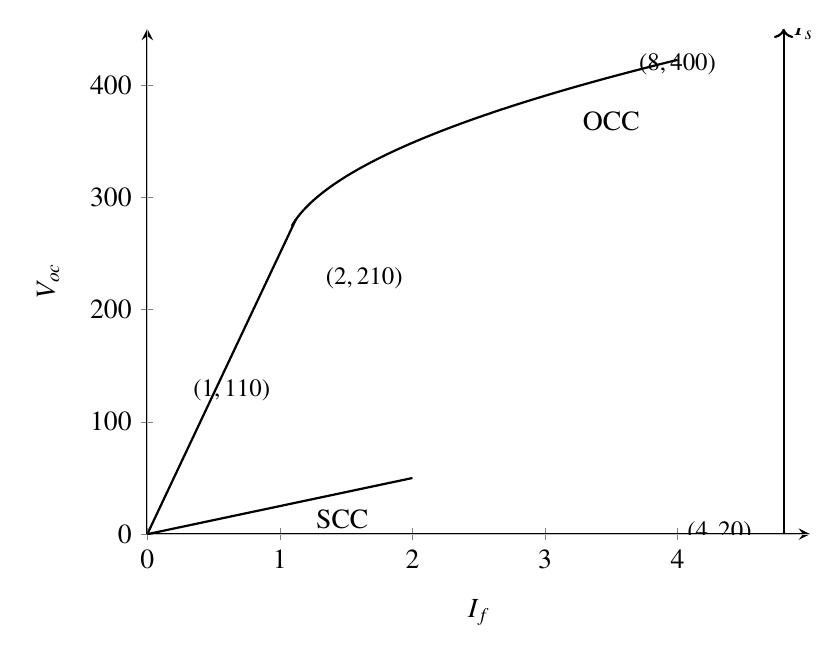
\begin{tikzpicture}
        \begin{axis}[
            axis lines = middle,
            xlabel = $I_f$,
            ylabel = $V_{oc}$,
            xmin = 0, xmax = 5,
            ymin = 0, ymax = 450,
            xtick = {0,1,2,3,4},
            ytick = {0,100,200,300,400},
            x label style={at={(axis description cs:1,0)},anchor=west},
            y label style={at={(axis description cs:0,1)},anchor=south},
            extra x ticks={0},
            extra y ticks={0},
            extra tick style={grid=major},
            axis line style=thick,
            xlabel near ticks,
            ylabel near ticks,
            every axis plot/.append style={thick},
            legend pos = north west,
            width=10cm, height=8cm,
        ]

        % Plot for OCC curve
        \addplot[domain=1.09:4, samples=100, smooth] {100*(x-1.03)^(0.5)+250};

        % Plot for SCC curves
        \addplot[domain=0:2, samples=2] {25*x};
        \addplot[domain=0:1.12, samples=2] {250*x};

        % Points with labels
        \node at (axis cs:0,0) [below left] {\small $(0,0)$};
        \node at (axis cs:0,10) [left] {\small $(0,10)$};
        \node at (axis cs:1,110) [above left] {\small $(1,110)$};
        \node at (axis cs:2,210) [above left] {\small $(2,210)$};
        \node at (axis cs:4,20) [below right] {\small $(4,20)$};
        \node at (axis cs:4,400) [above] {\small $(8,400)$};

        % Additional labels for OCC and SCC curves
        \node at (axis cs:3.5,350) [above] {OCC};
        \node at (axis cs:1.2,30) [below right] {SCC};

        % Right-hand axis line and label
        \draw[->, thick] (axis cs:4.8,0) -- (axis cs:4.8,450) node [right] {$I_{sc}$};

        % Top axis label for V_oc
        \node[above] at (axis cs:0,450) {$V_{oc}$};

        \end{axis}
    \end{tikzpicture}
   
  
    \end{figure}
    \begin{enumerate}
        \item 2.100
        \item 2.025
        \item 2.000
        \item 1.000
    \end{enumerate}

    \item Let $a_x$ and $a_y$ be unit vectors along $x$ and $y$ directions, respectively. A vector function is given by:
    $$
    \mathbf{F} = a_x y - a_y x
    $$
    The line integral of the above function 
    $$\int_C \vec{F} \cdot d\vec{l}$$

    
    along the curve $C$, which follows the parabola $y = x^2$ as shown below is {\underline{\hspace{1cm}}} (rounded off to 2 decimal places).
      \begin{figure}[H]
        \centering
        
    \begin{tabular}{cc}
        \toprule
        \( f \) (MPa) & Number of specimens with \\
                      & compressive strength equal to \( f \) \\
        \midrule
        23   & 4 \\
        28   & 2 \\
        22.5 & 5 \\
        31   & 5 \\
        29   & 4 \\
        \bottomrule
    \end{tabular}
  % Use the correct path to your Q4.tex file
    \end{figure}
   

    \item A resistor and a capacitor are connected in series to a 10 V dc supply through a switch. The switch is closed at $t = 0$, and the capacitor voltage is found to cross 0 V at $t=0.4\tau$, where $\tau$ is the circuit time constant. The absolute value of percentage change required in the initial capacitor voltage if the zero crossing has to happen at $t= 0.2\tau$ is {\underline{\hspace{2cm}}} (rounded off to 2 decimal places).
  

    \item A cylindrical rotor synchronous generator with constant real power output and constant terminal voltage is supplying 100 A current to a 0.9 lagging power factor load. An ideal reactor is now connected in parallel with the load, as a result of which the total lagging reactive power requirement of the load is twice the previous value while the real power remains unchanged. The armature current is now {\underline{\hspace{2cm}}}(rounded off to 2 decimal places).
   

    \item Bus 1 with voltage magnitude $V_1=1.1$ pu is sending reactive power $Q_{12}$ towards bus 2 with voltage magnitude $V_2 =1$ pu through a lossless transmission line of reactance $X$. Keeping the voltage at bus 2 fixed at 1 pu, the magnitude of voltage at bus 1 is changed, so that the reactive power $Q_{12}$ sent from bus 1 is increased by 20\%.Real power flow through the line under both the conditions is zero. The new value of the voltage magnitude, $V_1$, in pu  (rounded off to 2 decimal places), at bus 1 is {\underline{\hspace{2cm}}}.
          \begin{figure}[H]
        \centering
        
    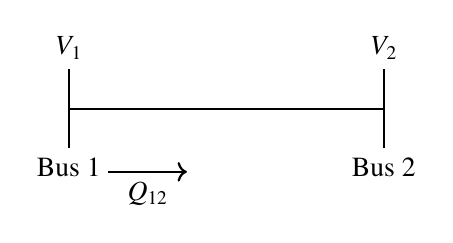
\begin{tikzpicture}
        % Draw the buses
        \draw[thick] (-2,0) -- (-2,1) node[above] {$V_1$};
        \draw[thick] (2,0) -- (2,1) node[above] {$V_2$};
        
        % Draw the line between the buses
        \draw[thick] (-2,0.5) -- (2,0.5);
        
        % Label the buses
        \node[below] at (-2,0) {Bus 1};
        \node[below] at (2,0) {Bus 2};
        
        % Draw the power flow arrow
        \draw[->, thick] (-1.5, -0.3) -- (-0.5, -0.3) node[midway, below] {$Q_{12}$};
    \end{tikzpicture}
     % Use the correct path to your Q4.tex file
    \end{figure}
       
   
    \item Windings 'A', 'B', and 'C' have 20 turns each and are wound on the same iron core as shown, along with winding 'X' which has 2 turns.The figure shows the sense (clockwise/anti-clockwise) of each of the windings only and does not reflect the exact number of turns. If windings 'A', 'B', and 'C' are supplied with balanced 3-phase voltages at 50 Hz and there is no core saturation, the no-load RMS voltage (in V, rounded off to 2 decimal places) across winding 'X' is {\underline{\hspace{2cm}}}.
     \begin{figure}[H]
        \centering
        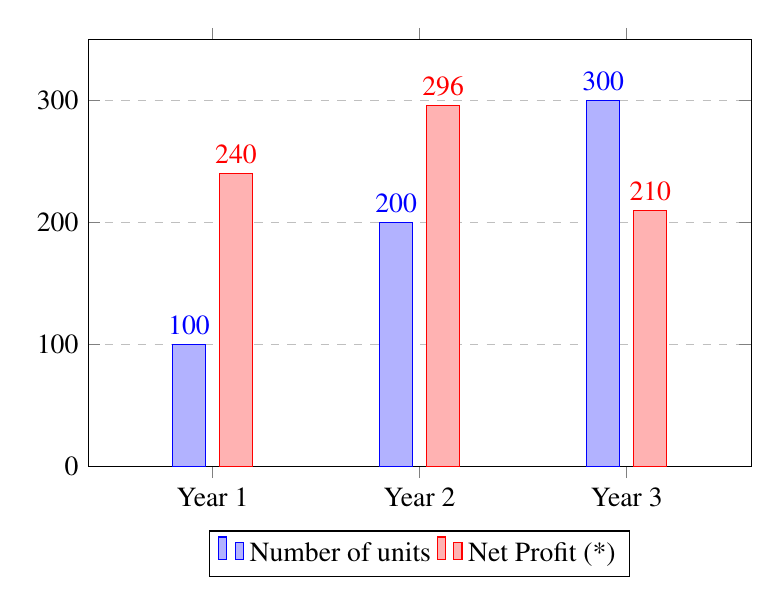
\begin{tikzpicture}
\begin{axis}[
    ybar=5pt,
    bar width=12pt,
    width=10cm, height=7cm,
    ymin=0, ymax=350,
    ylabel={},
    symbolic x coords={Year 1, Year 2, Year 3},
    xtick=data,
    nodes near coords,
    legend style={at={(0.5,-0.15)},anchor=north,legend columns=-1},
    enlarge x limits=0.3,
    ymajorgrids=true,
    grid style=dashed
]

\addplot coordinates {(Year 1, 100) (Year 2, 200) (Year 3, 300)};
\addplot coordinates {(Year 1, 240) (Year 2, 296) (Year 3, 210)};

\legend{Number of units, Net Profit (*)}

\end{axis}
\end{tikzpicture}  % Use the correct path to your Q9.tex file
    \end{figure}
    

    \item A cylindrical rotor synchronous generator has steady state synchronous reactance of 0.7 pu and subtransient reactance of 0.2 pu. It is operating at $(1 +j0)$ pu terminal voltage with an internal emf of $(1+j0.7)$ pu. Following a three-phase solid short circuit fault at the terminal of the generator, the magnitude of the subtransient internal emf (rounded off to 2 decimal places) is {\underline{\hspace{2cm}}} pu.
    
    \item In the dc-dc converter circuit shown, switch $Q$ is switched at a frequency of 10 kHz with a duty ratio of 0.6. All components of the circuit are ideal, and the initial current in the inductor is zero. Energy stored in the inductor in mJ (rounded off to 2 decimal places) at the end of 10 complete switching cycles is {\underline{\hspace{2cm}}}.
  
    \item A single-phase, full-bridge, fully controlled thyristor rectifier feeds a load comprising a 10 $\Omega$ resistance in series with a very large inductance. The rectifier is fed from an ideal 230 V, 50 Hz sinusoidal source through cables which have negligible internal resistance and a total inductance of 2.28 mH. If the thyristors are triggered at an angle $\alpha = 45^\circ$, the commutation overlap angle in degree (rounded off to 2 decimal places) is{\underline{\hspace{2cm}}}.
   

    \item A non-ideal Si-based pn junction diode is tested by sweeping the bias applied across its terminals from -5 V to +5 V. The effective thermal voltage, $V_T$, for the diode is measured to be (29 $\pm$ 2) mV. The resolution of the voltage source in the measurement range is 1 mV. The percentage uncertainty (rounded off to 2 decimal places) in the measured current at a bias voltage of 0.02 V is {\underline{\hspace{2cm}}}.
   

\end{enumerate}









\end{document}